The robot base comprises of four legs, with two on each side that are concentric. The robot arm that is attached has four degrees of freedom.


\begin{figure}[htb]
	\centering
	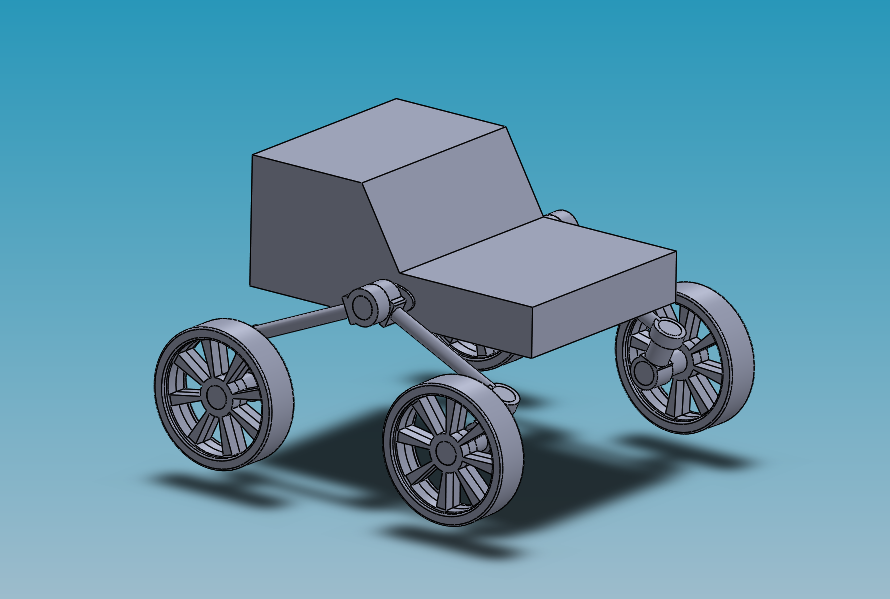
\includegraphics[scale=0.70]{sections/robot-design/images/SRR_model.png}
	\label{sample_return_rover:robot_design:srr_cad}
	\caption{Sample Return Rover in SolidWorks}
\end{figure}



\begin{figure}[htb]
	\centering
	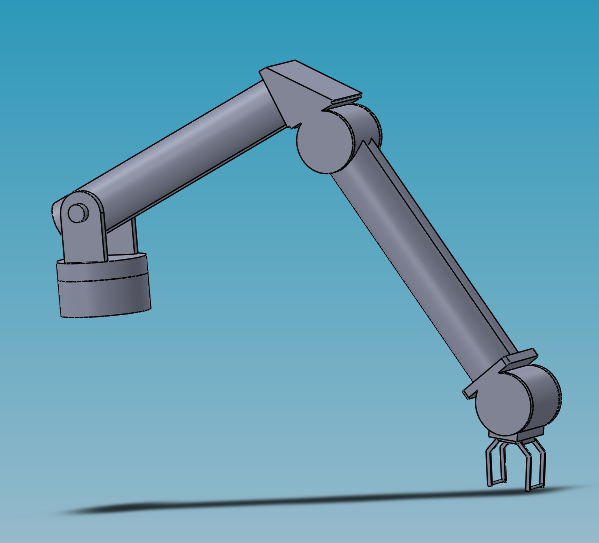
\includegraphics[scale=0.70]{sections/robot-design/images/arm_model.png}
	\label{sample_return_rover:robot_design:arm_side.png}
	\caption{Arm Model in SolidWorks}
\end{figure}


\begin{figure}[htb]
	\centering
	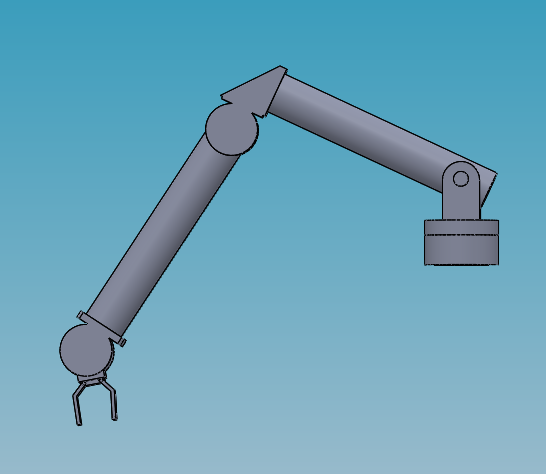
\includegraphics[scale=0.70]{sections/robot-design/images/arm_side.png}
	\label{sample_return_rover:robot_design:arm_side.png}
	\caption{Side View of Robot Arm}
\end{figure}
